\chapter{Performance Metrics of Program Execution}
\label{chap:efficiencyMetrics}

A widely-established metric to balance time and energy performance of a program execution is Energy-Delay Product (EDP) \cite{Venkat2014, Ratkovic2015, Kumar2003, Gonzalez1996} defined by:
%
\begin{equation}
\uprho = \mathsf{E} * \mathsf{T}^\mathsf{RT}
\end{equation}
%
where $\mathsf{E}$ is energy consumed by a processing unit for a program execution and $\mathsf{T}^\mathsf{RT}$ is program response time discussed below. EDP metric is similar to power-delay product (PDP) used in digital electronics\footnote{https://wikipedia.org/wiki/Power-delay\_product}.

\section{Time performance metrics}
\label{sec:timePerformanceMetrics}

The major time performance metric is program response time denoted by $\mathsf{T}^\mathsf{RT}$, which is the time from its invocation until completion. For example, in a non-preemptive scenario of Fig.~\ref{fig:nonPreemptiveExecution}, the program response time is 12, and in a preemptive in Fig.~\ref{fig:preemptiveExecution} it is 15 time units. In turn, $\mathsf{T}^\mathsf{RT}$ is subject to various other metrics, including preemption and migration overheads discussed in Section~\ref{sec:performanceOverheads}, latency and execution time, discussed next.

Consider a 3-blocks program execution in Fig.~\ref{fig:preemptiveExecution}. 
The time since program's release until its actual start is latency ($\Delta t^{\mathsf{l}}$), which is 2 time units in the figure. Next 4 time units are program's first block execution time, which is the time since a block start until its completion. The sum of all blocks execution times is program execution time ($t^{\mathsf{exec}}$). While, the sum of blocks preemption times is program preemption time ($t^{\mathsf{pm}}$), which is the time when the program is preempted by other programs. 

With these metrics we express program response time as:
%
\begin{equation}
\mathsf{T}^\mathsf{RT}=t^\mathsf{c}-t^\mathsf{r}=\Delta t^\mathsf{l}+\Delta t^\mathsf{pm}+\Delta t^\mathsf{exec}*1.25
\end{equation}
%
where $t^\mathsf{r}$ and $t^\mathsf{c}$ are program release and completion times.
We note that performance overheads are not yet considered. Instead, we assume that they take at most 25\% of program execution time.

\begin{figure}
\centering
\begin{subfigure}{.7\columnwidth}
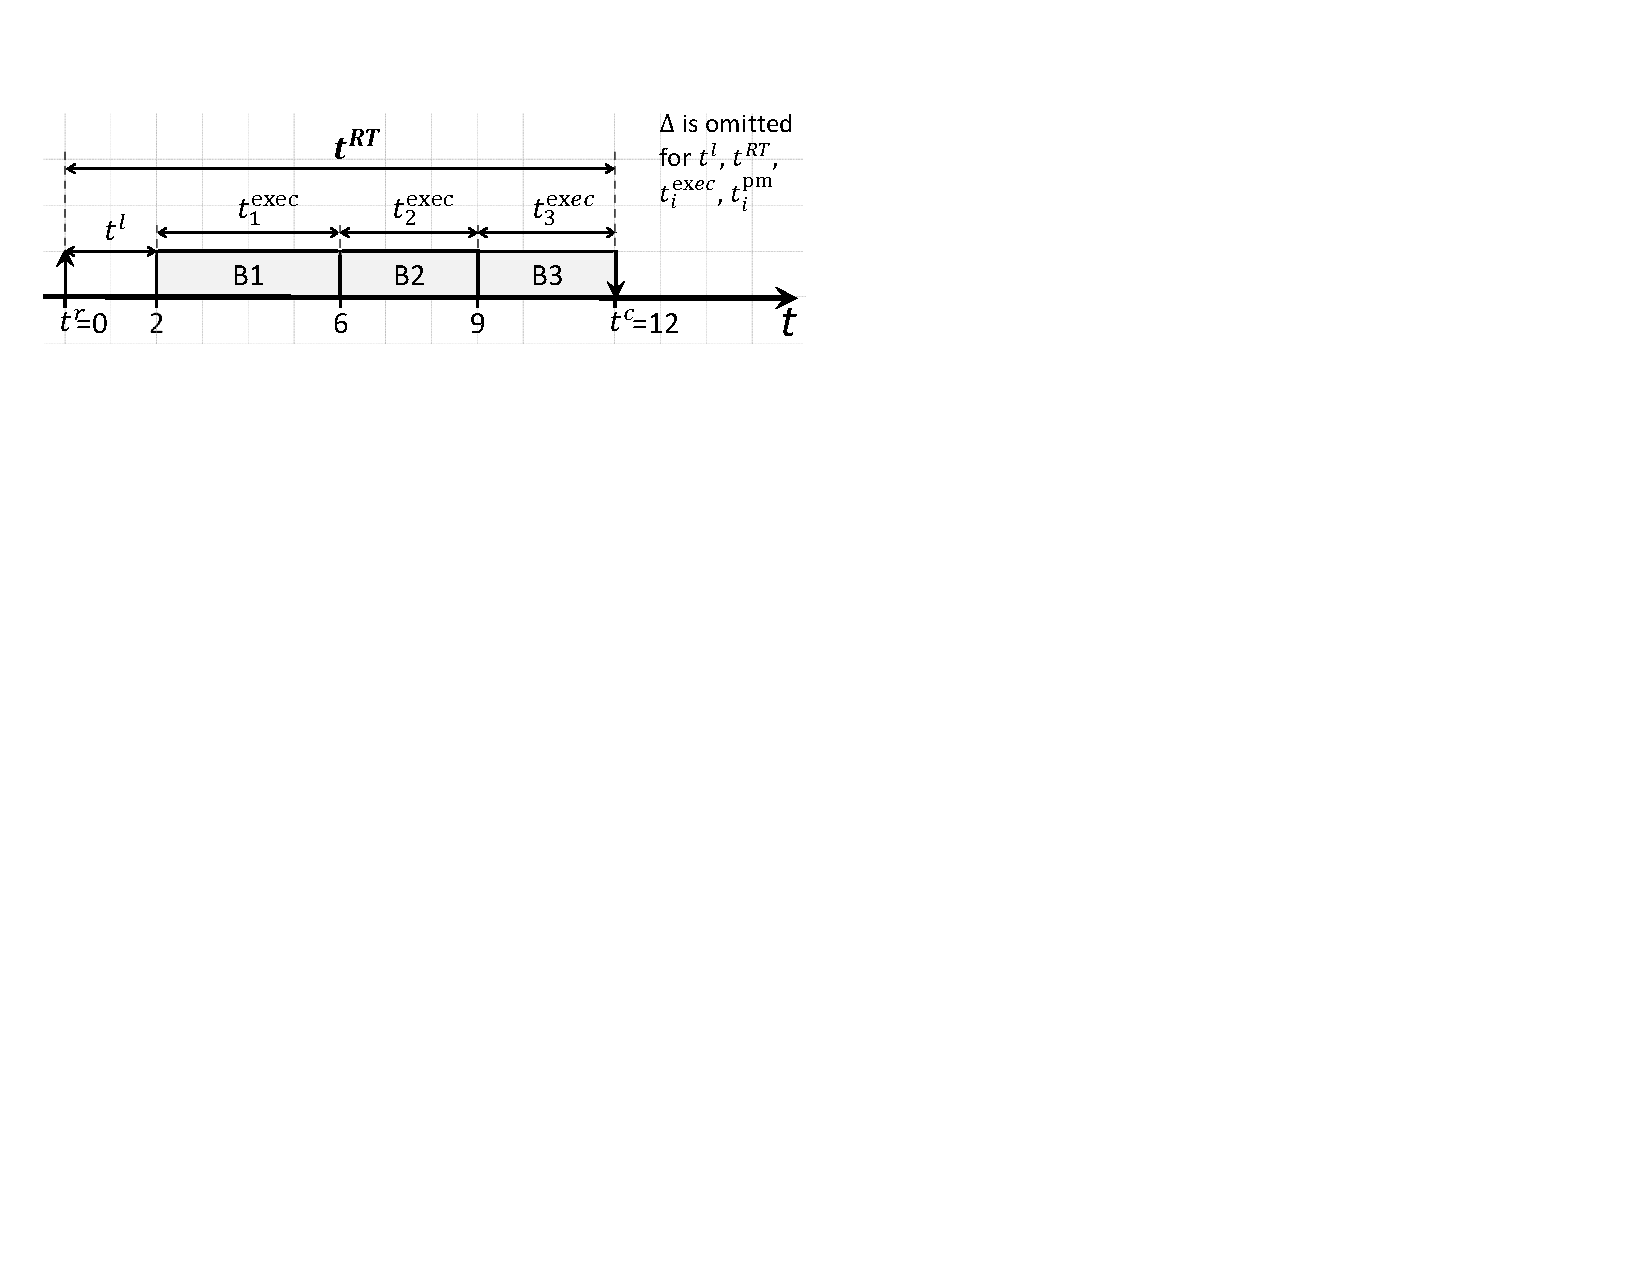
\includegraphics[width=\columnwidth]{figs/nonPreemptiveExecution.pdf}
\caption{Non-preemptive execution}
\label{fig:nonPreemptiveExecution}
\end{subfigure}
\begin{subfigure}{.7\columnwidth}
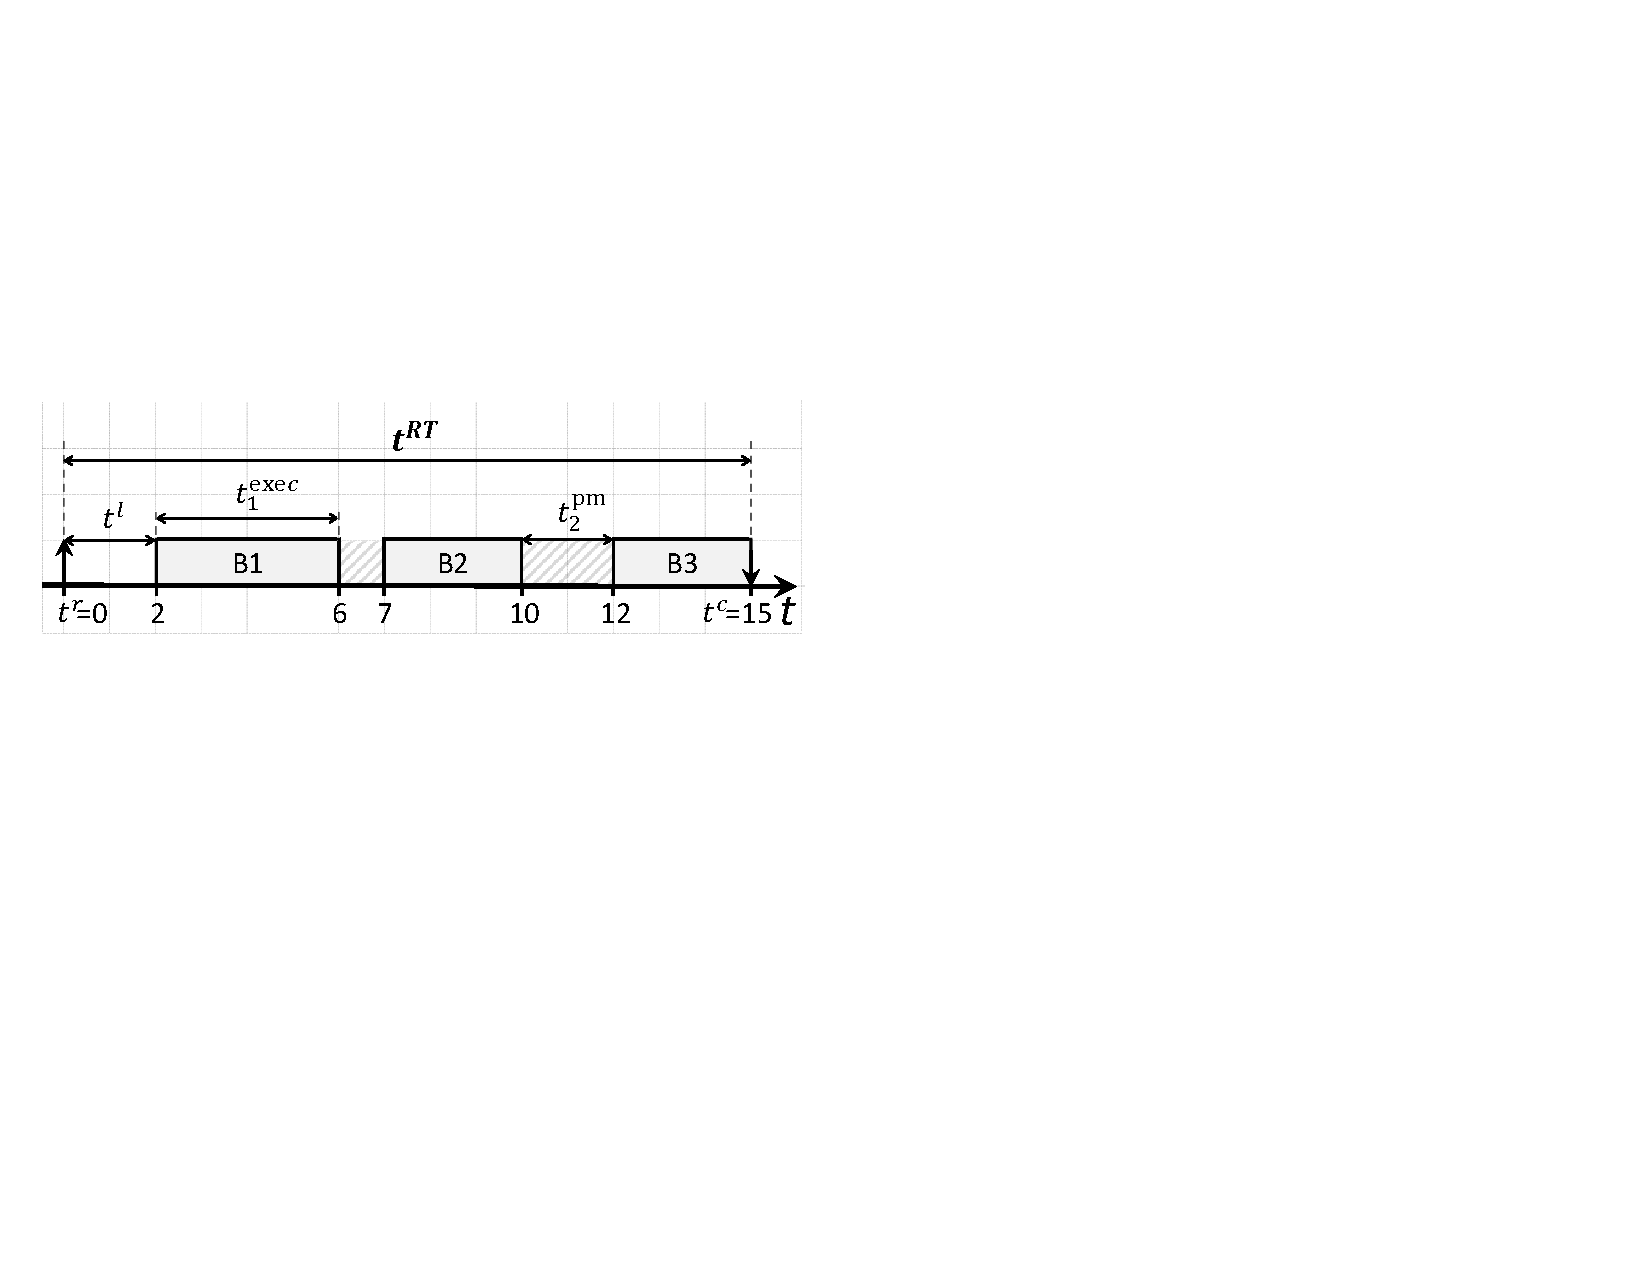
\includegraphics[width=\columnwidth]{figs/preemptiveExecution.pdf}
\caption{Preemptive execution at blocks completion}
\label{fig:preemptiveExecution}
\end{subfigure}
\caption{Time metrics of an N-blocks program execution}
\label{fig:executionMetrics}
\end{figure}

For our toy example, below in Fig.~\ref{fig:twoSchedulesExample} we compute average program response and execution times for two schedules. Notice that schedule S1 has higher average response time, but lower average execution time than S2. Also, S1 preemption time is twice larger than in S2. %In our extended example in Fig.~\ref{fig:s1PreemptionMigration} the total preemption times of Prog. P1, P2 and P3 are 3, 6 and 0 time units correspondingly.

\section{Energy performance metrics}
\label{sec:energyConsumption}

Nowadays energy efficiency deserves attention and is considered equally with program response time. However, unlike response time, energy consumption is difficult to measure. Typical direct measurement approaches with specialized devices, such as wattmeter and multimeter, which are attached to an operating hardware, are often impracticals. This motivates the development of theoretical techniques to model energy consumption. This modeling mostly relies on the analysis of different program execution events collected from the following sources\footnote{https://www.brendangregg.com/perf.html}:
\begin{itemize}
\item Hardware: Performance monitor counters (PMCs);
\item Operating system: Kernel counters and tracepoints;
\item Tracing: Dynamic instrumentation of user-level software.
\end{itemize}
Specifically, PMC represented as registers collect statistics of CPU and memory units. While tracing in software collects the statistics on a higher level program execution. Then, this statistics, such as number of clock cycles, integer or floating point instructions, branch mispredictions, cache misses, page faults, context switches and migrations, is aggregated into a value representing energy consumption of a program execution. Some studies expect that a modeling error is within 5-10\% compared to the direct measurements\cite{Joseph2001, Brooks2000} or cycle-accurate simulation \cite{Li2003}.

Energy consumption denoted by $\mathsf{E}$ is defined by:
%
\begin{equation}
\mathsf{E} = \mathsf{P} * \mathsf{T}^\mathsf{RT}
\end{equation}
%
where $\mathsf{P}$ is average power in Watts used by hardware for a program execution, and $\mathsf{T}^\mathsf{RT}$ is program response time in seconds. Hence, $\mathsf{E}$ is measured in Watt-seconds, which are actually Joules denoted by $\mathsf{J}$.

Moreover, various other energy performance metrics are available, such as Energy per Instruction (EPI), Energy per Operation (EPO), which are however not yet considered in our analysis. 
	
	
\section{Optimization objective}
\label{sec:energyDelayProduct}
\label{sec:optimizationObjective}

Our key optimization objective is a so-called Energy-Delay Product (EDP) metric \cite{Ratkovic2015, Gonzalez1996}, which we denote by $\uprho$. It aggregates both time and energy performance metrics of all executing programs

For an individual program EDP is computed by:
%
\begin{equation}
\uprho = \mathsf{E} * \Delta t^\mathsf{RT}
\end{equation}
%
Here, both energy and time are considered equally, while in alternatives to $\mathsf{EDP}$, such as $\mathsf{ED^2P}$ or $\mathsf{ED^3P}$, time is critical:
%
\begin{equation}
\uprho^2 = \mathsf{E} * \Delta t^{\mathsf{RT}^2}
\end{equation}
%
%
\begin{equation}
\uprho^3 = \mathsf{E} * \Delta t^{\mathsf{RT}^3}
\end{equation}
%

Consider in Fig.~\ref{fig:EDPExample}, which depicts energy consumption vs. average program response of three abstract schedules. Schedule 1, represented as a dark square, has EDP of 300 Joules-second, which is indicated by the hyperbolic dashed-line. While schedules 2 and 3, represented by two lighter circles, have equal EDP of 150. Note the difference in ratios of times to energy between schedule 1-2 and 3-2. Compared to schedule 1, the execution time of schedule 2 increased less than energy consumption decreased. While between schedules 2 and 3 these time/energy ratios are the same. Hence, schedules 2 and 3 are equal and better than schedule 1 from the EDP-perspective.

The EDP metric is extensively used later in our analysis starting from Section~\ref{sec:schedulingProcedure}.

%Also, we compute $\mathsf{EDP}$ in Fig.~\ref{fig:programsEDP} for each program of both schedules S1 and S2 in Fig.~\ref{fig:twoSchedulesExample}. Note the difference in 92 and 71\% for Prog. P2 and P3, which indicates that schedule S2 is significantly more efficient than S1.


\begin{figure}
\centering
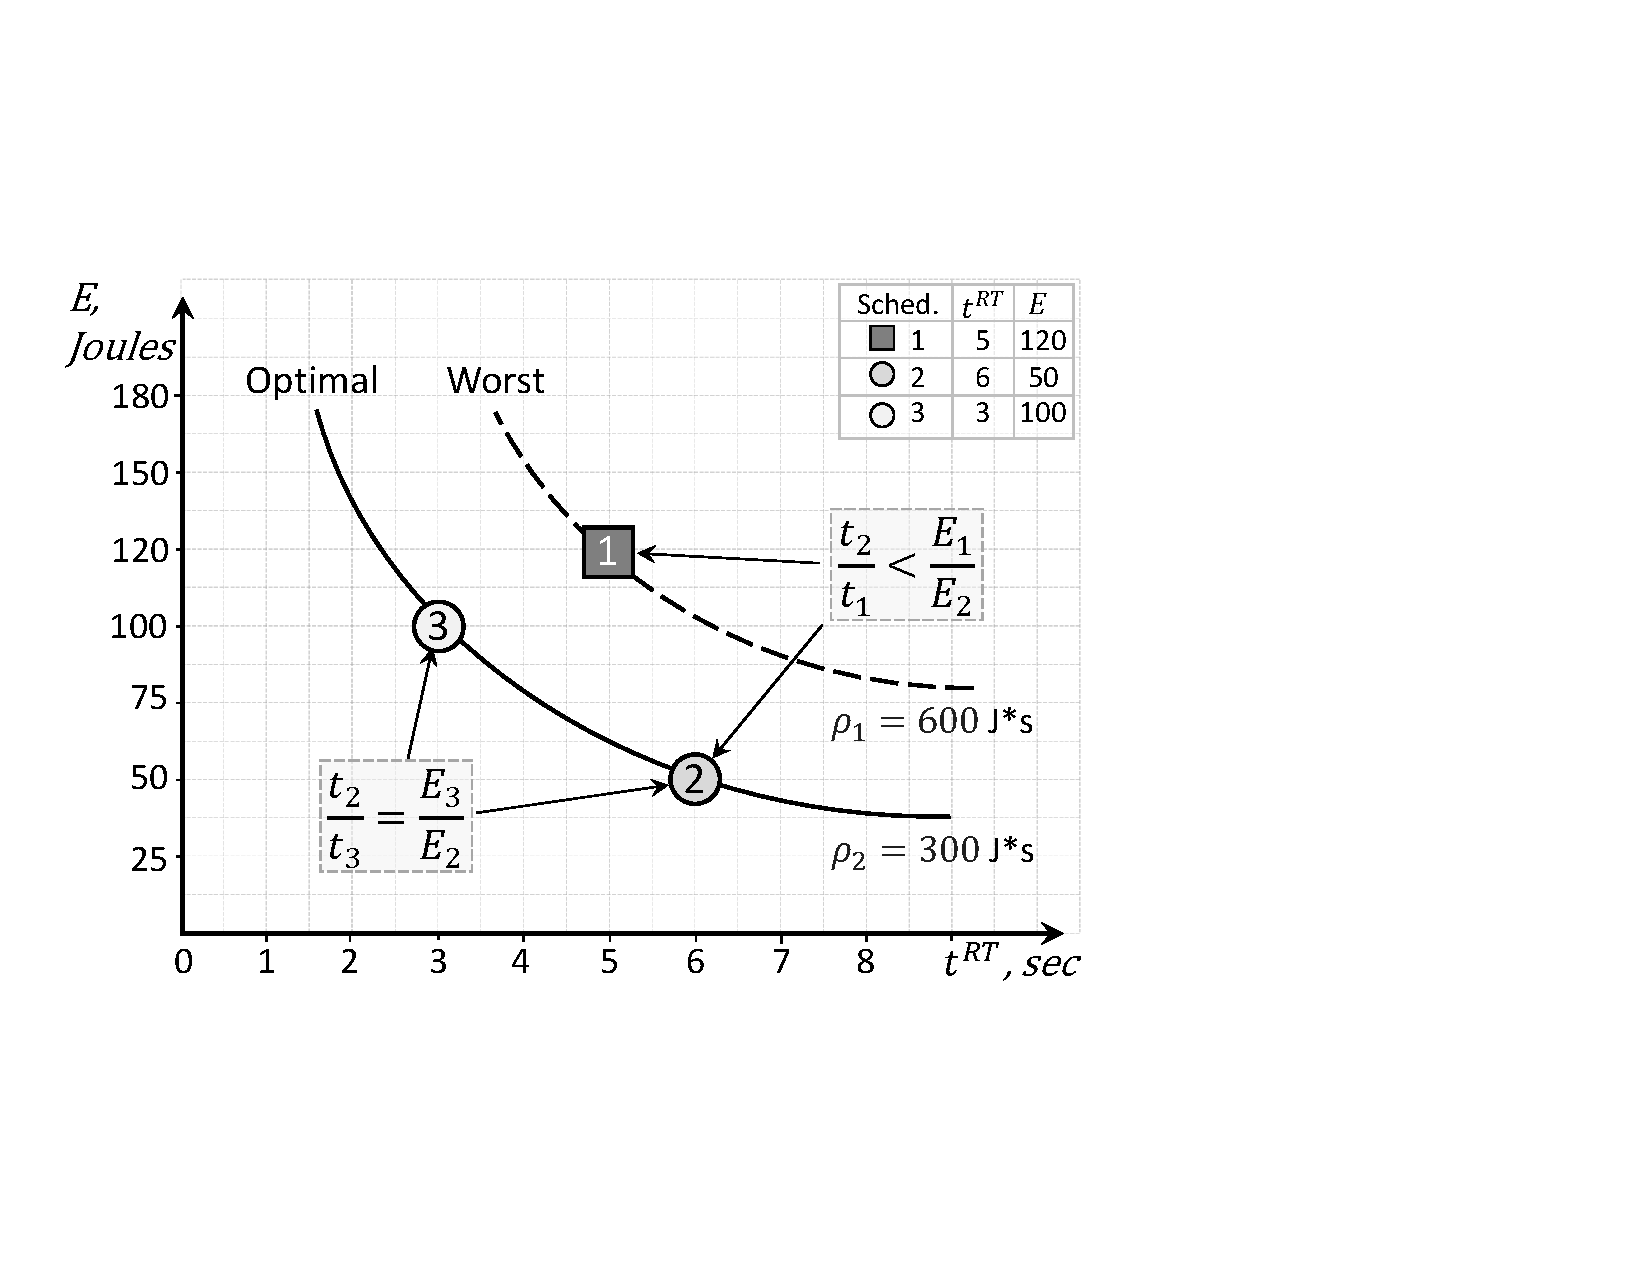
\includegraphics[width=.7\columnwidth]{figs/EDPExample.pdf}
\caption{Trade-off between response time and energy consumption. An optimal line (Sched. 2 and 3) has better trade-off.}
\label{fig:EDPExample}
\end{figure}

%\section{Existing heterogeneous schedulers}
%\label{sec:existingSchedulers}

%\todo{To list 2-3 publicly available implementations of a heterogeneous scheduler, discussing their flaws, consideration of overheads, choice of scheduling objective and energy-awareness}


